\documentclass[titlepage]{article}
\usepackage{tikz}
\usetikzlibrary{shapes.geometric, arrows}

% tikz styling
\tikzstyle{block} = [rectangle, 
			draw, 
			rounded corners, 
			text centered, 
			text width = 5em, 
			minimum height = 2em]

\title{Networks Lab Report\\Assignment 2}
\author{Md Sahil\\BCSE III\\Roll-001710501029}
\date{}

\begin{document}

{\maketitle}

\section{Objectives}
Implement three data link layer protocols, 
Stop and Wait, 
Go Back N Sliding Window 
and Selective Repeat Sliding Window for flow control.

\section{Design and Implementation}
\subsection{Purpose of the program}

\subsection{Program structure}
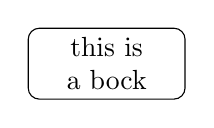
\begin{tikzpicture}[node distance = 1 cm]
\node [block] (start) {this is a bock};
\end{tikzpicture}

\subsection{Code snippets}

\section{Test cases and Results}

\end{document}
